
%%%%%%%%%%%%%%%%%%%%%
\section{Champ électrique et potentiel scalaire}
%%%%%%%%%%%%%%%%%%%%%
%
Le champ électrique créé par une particule chargé s'étend dans l'espace à 3 dimensions. Il est possible, afin de simplifier les schéma de se limiter à 2 dimensions.

Le champ électrique créé par une particule chargée est radial et son amplitude décroit avec la distance à la particule.

\begin{center}
\tikzstyle{fleche}=[->,line width=1pt]
\begin{tikzpicture}
  \begin{scope}[xshift=0 cm,yshift=0 cm, scale = 1.6]%
\foreach \t in {60,120, ...,360}
\draw [fleche] (\t:1) -- (\t:2.8);
\foreach \t in {30,90, ...,360}
\draw [fleche] (\t:2) -- (\t:2.45);
\foreach \t in {15,45,-15,-45}
\draw [fleche] (\t:3) -- (\t:3.2);
\foreach \t in {15,45,-15,-45}
\draw [fleche] (\t+180:3) -- (\t+180:3.2);
\draw [fill=red] (0,0) circle(0.1) node [above right] {$Q_1$};
  \end{scope}
\end{tikzpicture}
\end{center}


Comme le champ de pente dérive d'un champ scalaire (le champ d'altitude), le champs electrique dérive d'un champ scalaire. On l'appelle le potentiel électrique. On représente ci-dessous les lignes de même potentiel (équi-potentiel) du potentiel électrique créé par une particule chargée.

\begin{center}
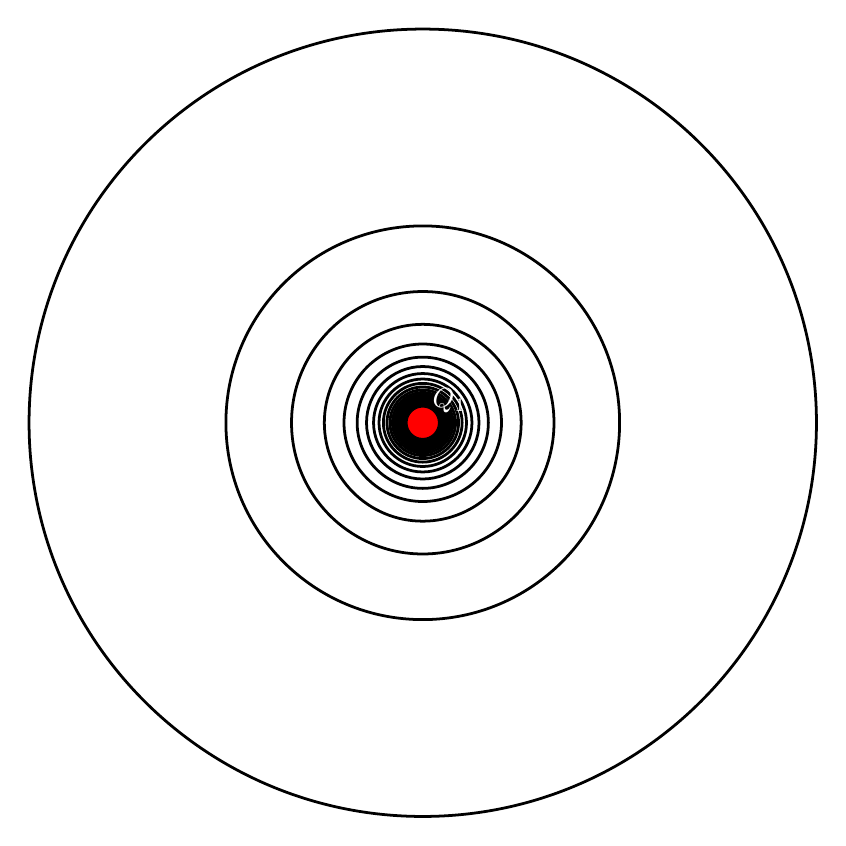
\begin{tikzpicture}
  \begin{scope}[xshift=0 cm,yshift=0 cm, scale = 1]%
\foreach \t in {1,2, ...,30}
\draw [line width=1pt] (0,0) circle (5/\t) ;

\draw [fill=red] (0,0) circle(0.2) node [above right,text=white] {$Q_1$};
  \end{scope}
\end{tikzpicture}
\end{center}

En 3 dimensions, les points de même potentiel sont des surfaces. Les surfaces équi-potentiel du potentiel créé par une particule chargée sont des sphères.

%%%%%%%%%%%%%%%%%%%%%%%%%%%%%%%%%%%%%%%%%%%%%%%%%%%%%%%%%%%%%%%%%%%%%%%%%%%%
